\documentclass{article}
\usepackage{algorithmicx}
\usepackage{algpseudocode}
\usepackage{graphicx}
\usepackage[utf8]{inputenc}
\usepackage{color}
\usepackage{mathtools}

\begin{document}

%{\noindent \Huge Problema a resolver: Puentes sobre lava caliente}
%\newline \newline 
\textbf{Experimento 1.1 - análisis del código generado}\newline
a)Porque en el MakeFile se usa -g (incluye en el ejecutable generado la información necesaria para poder rastrear los errores usando un depurador, tal como GDB) y esto hace que se muestren funciones de debugg.\newline
b) Las variables locales se manipulan con la pila, por ejemplo usa indices para recorrer la matriz, entonces tiene que estar actualizando por la iteración por la que va en la pila.\newline
Esto ocupa muchas líneas de código, lugar en la pila(ya que no es necesario usarla siendo que existe los registros de propósito general) y es lento. \newline
c) En lugar de utilizar la pila para manejar todas las variables locales, se podrían usar registros(ahorrando muchas accesos a memoria que son "caros").\newline
Además guarda datos en la pila que nunca vuelve a usar, usa add para sumar 1 a variables en la pila en vez de usar inc y en vez de usar lea usa imul.
También hace swaps de variables para poner el mismo valor que tenían.
\newline


\textbf{Experimento 1.2 - optimizaciones del compilador}\newline

a) Ultiliza los registros para manejar las variables locales , saca las que están en la pila a un registro. 
Como no tiene que estar actualizando la pila todo el tiempo hay menos líneas de código y el espacio en la pila no se desperdicia. 
Ahora al no usar la pila para manejar las variables locales no guarda cosas innecesarias que nunca vuelve a usar.\newline
Además usa lea en vez de imul.\newline
b) Además del 01 que es el flag que utilizamos para este experimento, exiten otros como O0(reduce el tamaño del código y tiempo de ejecución), O2 ,O3 y ofast entre otros.\newline
El flag O0 reduce el tiempo de compilación.
El flag -O1 optimiza en espacio, si hay optimizaciones que aumentan el tamaño tambien las va a omitir.\newline
El flag -O2 optimiza en velocidad se reemplazan instrucciones que demoran mas por otras que no lo hacen.\newline
El flag -O3 utiliza vectorización entre otras cosas. \newline

c) Paralelización automática, eliminación de código muerto y Evaluación perezosa.


\newpage

\textbf{Experimento 1.3 - calidad de las mediciones}\newline
e)Todos los datos obtenidos son corriendo cropflip(./tp2 cropflip -i c lena.bmp 400 400 0 0) versión asm y c respectivamente, obteniendo la esperanza de correr 500 veces el algoritmo, luego obtengo la esperanza y varianza de hacer esto 10 veces.
\newline
Cuando menciono ciclo sin fin es que mientras corro el algortimo de cropflip de la manera mencionada arriba, corro también en 4 consolas(una por core lógico) un programa que cicla infinitamente sumando 1 a una variable.
\newline

En ASM: 
\newline

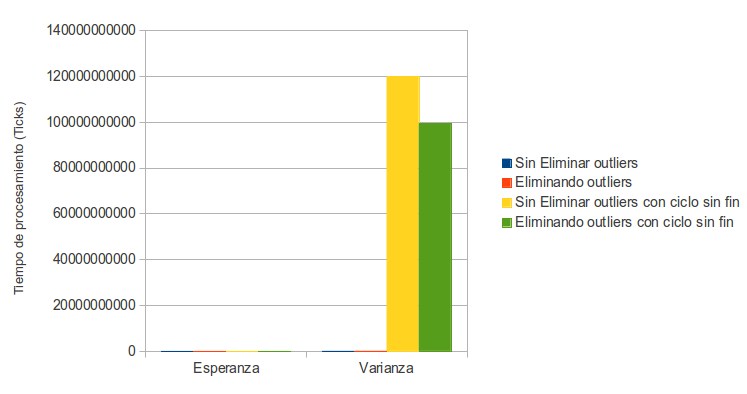
\includegraphics[width=\textwidth,height=\textheight,keepaspectratio
]{graficoasm.png}
\begin {flushleft}
\end{flushleft}
\vspace{0.4cm}
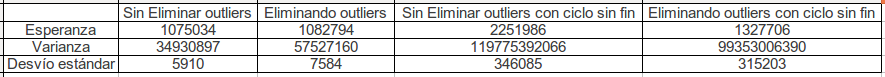
\includegraphics[width=\textwidth,height=\textheight,keepaspectratio
]{tablaASM.png}
\begin {flushleft}
\end{flushleft}
\newpage
En C: \newline
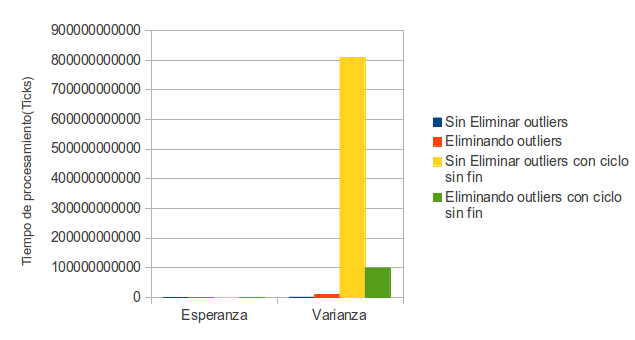
\includegraphics[width=\textwidth,height=\textheight,keepaspectratio
]{graficoC.png}
\begin {flushleft}
\end{flushleft}
\vspace{0.4cm}
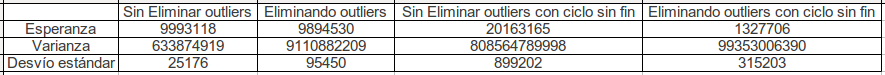
\includegraphics[width=\textwidth,height=\textheight,keepaspectratio
]{tablaC.png}
\begin {flushleft}
\end{flushleft}


Como podemos observar cuando corremos el ciclo sin fin la varianza aumenta, y cuando sacamos los ouliers la varianza disminuye.\newline
Esto se debe a que los resultados que obtenemos cuando corremos el ciclo sin fin tienen "picos altos y bajos muy marcados" y al eliminarlos la varianza baja notablemente.
\newpage

\textbf{Experimento 1.4 - secuencial vs. vecorial}\newline
e)
\vspace{0.4cm}
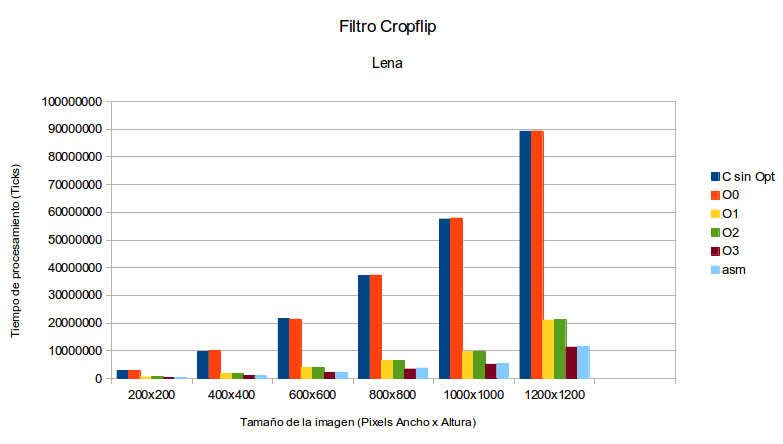
\includegraphics[width=\textwidth,height=\textheight,keepaspectratio
]{graficoOpt.png}
\begin {flushleft}
\end{flushleft}
Una tabla con la esperanza: \newline
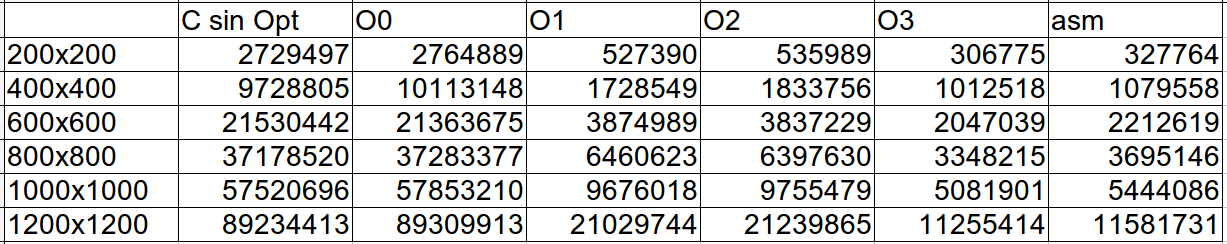
\includegraphics[width=\textwidth,height=\textheight,keepaspectratio
]{tablaEsperanzaOpt.png}
\begin {flushleft}
\end{flushleft}

Una tabla con el desvío estándar:\newline
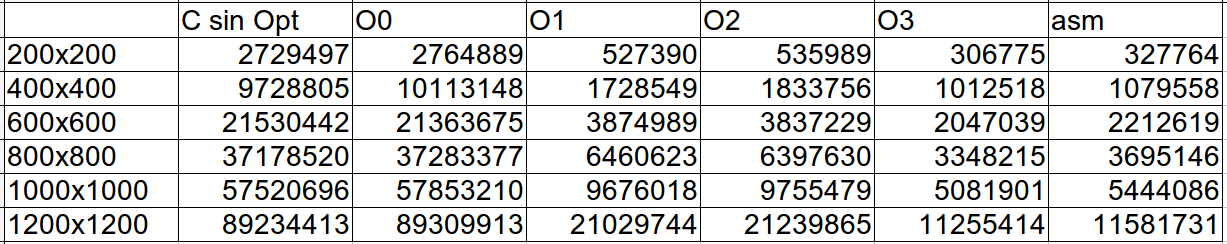
\includegraphics[width=\textwidth,height=\textheight,keepaspectratio
]{tablaEsperanzaOpt.png}
\begin {flushleft}
\end{flushleft}

Intuitivamente creíamos que ninguna optimización podría ganarle a la implementación de asm porque esta utiliza operaciones SIMD que permiten manejar más cantidad de datos en 1 operación, pero O3 le gana.
Esto es porque utiliza vectorización, y operaciones que tienen menor "costo" que las que usamos nosotros en asm.
La optimización O3 es lo suficientemente "inteligente" como para traducir el código c a asm usando SIMD, ganandole en tiempo de ejecución a nuestra implementación en asm.\newline
De todos modos la diferencia en performance es mínima. \newline
Se puede observar a simple vista que la implementación de c sin optimizaciones (o con O0) tiene una performance muy mala en comparación con la de asm y las optimizadas.
Como mencionamos en el experimento 1.1, el flag O1 optimiza el espacio, entonces la performance no se ve afectada prácticamente.
El flag O2 cambia intrucciones lentas por otras más rápidas, en este caso se ve que el tiempo de ejecución se redujo a más de la mitad al igual que con el flag O2.
Con el flag no hay diferencia porque solo acota el tiempo de compilación.
Y finalmente el flag O3 reduce drásticamente el tiempo de ejecución. 
\newline

\textbf{Experimento 1.5 - cpu vs. bus de memoria}\newline
Intuitivamente los accesos a memoria son mas caros que las operaciones lógicas y las aritméticas, veamos que sucede con los gráficos.
\newline
Usando add, subb, shl shr con rax (porque no está ocupado por el código) para las instrucciones aritméticas/ lógicas
y lecturas y escrituras en las matrices de entrada y salida.\newline
Usando la pila también cumplía el objetivo de agregar "instrucciones de memoria" pero accediendo a disco es mucho más evidente el costo.\newline
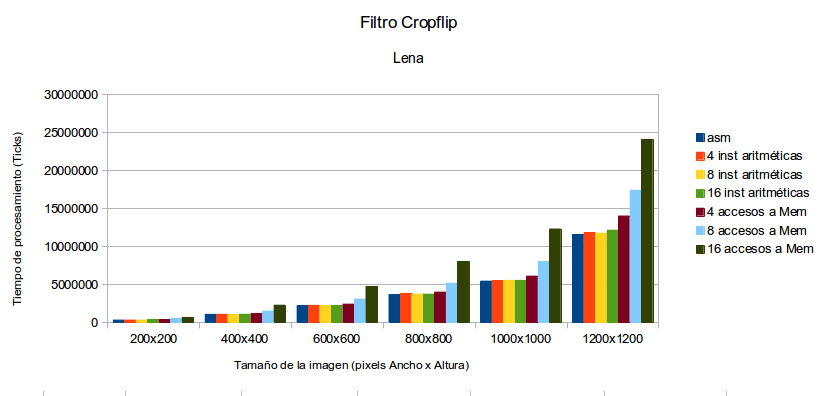
\includegraphics[width=\textwidth,height=\textheight,keepaspectratio
]{graficoMenVsArit.png}
\begin {flushleft}
\end{flushleft}

Una tabla con la esperanza: \newline
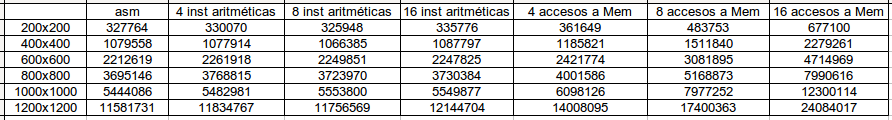
\includegraphics[width=\textwidth,height=\textheight,keepaspectratio
]{tablaMenVsArit.png}
\begin {flushleft}
\end{flushleft}

Una tabla con el desvío estándar:\newline
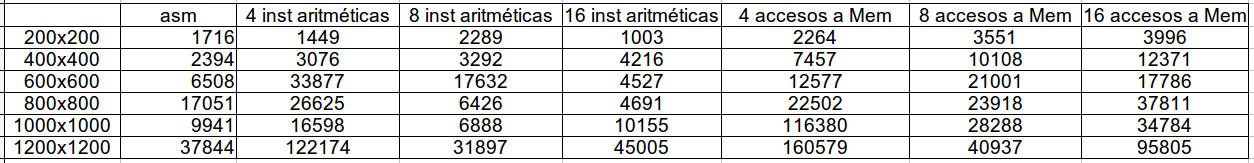
\includegraphics[width=\textwidth,height=\textheight,keepaspectratio
]{tablaVarianzaMenvscpu.png}
\begin {flushleft}
\end{flushleft}
Como vemos en el gráfico cuando aumentamos la cantidad de accesos a memoria, el tiempo de ejecución se ve afectado negativamente, es mucho más lento.
En cambio cuando agregamos instrucciones aritmeticas el cambio en performance es mínimo.
Con lo cual podemos concuir que los accesos a memoria son el factor que limita la performance.

\textbf{informe de cropflip en ASM}\newline

En rdi tengo el puntero a la matriz de entrada y en rsi tengo el puntero a la matriz de salida.\newline
Primero vamos a pone src (rdi) en la fila offsety ([rbp +40]). \newline
Para esto vamos a hacer un ciclo que haga tantas iteraciones como el valor de offsety.\newline
En cada paso del ciclo vamos a sumar src con src\_row\_size(r8d) 
para poder mover el puntero a la siguiente fila.

Luego vamos a poner dst(rsi) en la última fila.
Para esto vamos a hacer un ciclo de tamy-1 iteraciones.
En cada iteración vamos a sumar a rsi con dst\_row\_size para poder mover el puntero a la siguiente fila.

Como tamx es la cantidad de pixels, quiero que tamx sea la cantidad de bits,  con lo cual, multiplico tamx * 4(cantidad de bits de un pixel) 

Como offsetx es la cantidad de pixels, quiero que offsetx sea la cantidad de bit, entonces voy a multiplicar a offsex por 4.

Voy a iterar las filas de la matriz de entrada, cuya cantidad es tamy.\newline
Ahora voy a hacer un ciclo por cada fila de la matriz de entrada (cituada al principio en offsety) hasta tamx.\newline
Tomo 4 pixels (16 bits) de la posición de memoria rdi+offsetx en un registro xmm y los voy a poner en la posición de memoria rsi.\newline
Avanzo 4 pixels el puntero de rdi y el de rsi. \newline
Cuando termino una fila,muevo el puntero que está en rdi a la siguiente fila en la matriz de entrada(sumando src\_row\_size a rdi) y subo una fila en la matriz de salida(restando dst\_row\_size a rsi).\newline

\textbf{informe de cropflip en C} \newline

Realizamos 2 fors anidados con indices i y j, filas y columnas respectivamente. Con i $\in$ \{0,tamy-1\} y k $\in$ \{0, (tamx*4)-1\} \newline
Voy a hacer un pasaje de a un pixel.
En la matriz de salida en la fila i columna j voy a poner el pixel de la matriz de entrada en la fila tamy + offsety -i -1, columna offsetx*4 +j. 
\newline

\textbf{Concluciones}\newline
Podemos concluir varias cosas, primero escribir código en C es cómodo e intuitivo. En cambio, escribirlo en ASM no es nada trivial, encontrar errores es difícil, hay que tener conciencia de como se maneja lo que estamos leyendo en memoria y donde se escribe.

Sin embargo se puede ver claramente en las experimentaciones  que el tiempo de ejecución de las implementaciones en asm es mucho mejor que las de c.
Lo cual era esperable dado que procesamos muchos datos a la vez y solo hacemos accesos a memoria dentro de
los ciclos para cargar los pixels de la imagen fuente y para escribirlos luego de procesarlos.

En cuanto al compilador se puede observar que cuando no tiene optimizaciones los algoritmos corren lento(en comparación con asm), y cuando se agregan los flags de optimizaciones los algoritmos corren a una diferencia más que notable. \newline
Incluso en cropflip el flag O3 supera mínimamente en performance a la implementación en asm, lo que nos llamó mucho la atención. 

%\includegraphics[width=\textwidth,height=\textheight,keepaspectratio
%]{ejemplopuente1.jpg}
%\begin {flushleft}
%En este ejemplo, \textit{$n = 10$} y el puente se escribe como 10 c 0 1 0 0 1 1 0 1 1 1.
%\newline Si \textit{$c = 3$}, entonces la soluci\'on est\'a dada por caer en los tablones 4 7 11. Notar que en realidad no existe un trabl\'on numerado con el 11, pero cuando exista una soluci\'on, para indicar que llegamos al punto de llegada, diremos que saltamos a un tabl\'on mayor estricto que la cantidad de tablones del puente (o sea, que estamos efectivamente fuera del puente).
%Si tuvieramos el mismo puente pero con \textit{$n = 2$}, claramente no existir\'ia una soluci\'on ya que, si bien podr\'iamos llegar al tabl\'on 7 sin problemas, una vez ah\'i no tendr\'iamos manera de saltar el 8, 9 y 10 que est\'an rotos.\end {flushleft}
%\vspace{1cm}
\end{document}